\documentclass[a4paper]{article}

\usepackage[english]{babel}
\usepackage[utf8]{inputenc}
\usepackage{amsmath}
\usepackage{graphicx}
\usepackage[colorinlistoftodos]{todonotes}
\usepackage{longtable}
\usepackage[toc,page]{appendix}

\title{The Effect of State Merit Aid on Choice of College Major}

\author{Tyler Remick and Poornima Joshi}

\date{\today}

\begin{document}
\maketitle

\begin{abstract}
Enter a short summary here. What topic do you want to investigate and why? What experiment did you perform? What were your main results and conclusion?
\end{abstract}

\section{Introduction}
\label{sec:introduction}

As a first-order attempt to remain competitive in the market for their best and brightest graduates, state policy makers have implemented State-Financed Merit-Based Scholarships (SFMBS). Research has shown that graduates are more likely to pursue employment in the same state in which they graduated from college  \cite{nano3}, and SFMBS programs incentivize students to remain in State for college. However, there may be unintended consequences of SFMBS programs that may put states in a worse position than in the absence of these programs. 

SFMBS programs award scholarships for in-state colleges and universities to students that meet certain GPA, standardized test, and/or class rank thresholds. The magnitudes of the awards vary by State, but range from a few hundred dollars to full-tuition waivers. The increasing ubiquity of these programs has garnered much attention among economists, particularly surrounding the effect of SFMBS programs on college outcomes such as persistence, completion, and post-college retention. Additionally, research has explored the effects on college enrollment, as well as the effect on the student’s enrollment in STEM degrees. However, the impact of SFMBS programs on choice of college major has not been explored. 

Exploring the impact of SFMBS programs on choice of college major is important for several reasons. First, estimating the effect of SFMBS on student’s choice of major will illuminate the preferences of college students over the set of college majors. This will allow us to identify the set of college majors that are normal goods, which I refer to as consumption-based majors, and the set of college majors that are inferior goods, which I refer to as investment-based majors. Understanding which degrees are viewed as an investment and which ones are viewed as consumption will better inform future policy measures. Second, estimating the effects of SFMBS on labor market outcomes is the best way to identify the success or failure of these programs and whether or not these programs should continue and be adopted in more states; adjusted and reapplied; or cease to exist altogether.


\section{Conceptual Framework}
\label{sec:theory}

There are at least three reasons why students will change their enrollment decisions as a result of SFMBS. The first are the annual renewal requirements that are inherent upon accepting an SFMBS scholarship. These requirements may include maintaining a certain overall GPA and/or enrolling in a particular number of credits. Since certain majors are more rigorous than others, the presence of these renewal requirements may induce students to enroll in less-rigorous major. The other two are concerned with income and substitution effects.

The income effect should be apparent: SFMBS are an in-kind transfer of income, as a result, students that receive SFMBS will experience an outward shift in their budget constraint, giving them a greater command over all other goods - income that was previously spent on higher education can now be spent on all other goods. The corresponding effect on a SFMBS recipients’ choice of major depends on their preferences over the set of college majors. Majors that are viewed as inferior will experience a decrease in enrollment, while majors that are viewed as normal will experience an increase in enrollment. 

The substitution effect may not be as apparent. As a result of SFMBS, the cost of a college education has been reduced. This effectively changes the relative returns across majors. Table 1 is a simplified, hypothetical illustration of this effect. This has been assumed to have two different majors: low-earnings and high-earnings majors. The table assumes that tuition and fees for a four-year college education is \$100,000; the expected lifetime earnings less the cost of the education, or net present value (NPV), of a low-earnings majors is \$400,000, while the NPV of a high-earnings major is \$1,400,000. The introduction of SFMBS programs changes the NPV of lifetime earnings to \$500,000 and \$1,500,000, respectively, because the student is no longer responsible for the cost of the education. As a result, the Lifetime Income Ratio (LIR) between the majors changes from 3.5 to 3.0 in states that offer SFMBS programs. This makes low-earnings majors relatively more attractive and should make high-earnings majors relatively less attractive. 

To summarize, the introduction of SFMBS will induce students to change majors due to annual renewal requirements, income effects, and substitution effects - the annual renewal requirements will induce students to enroll in less-rigorous majors; the income effect will induce students to choose majors with more stimulating curriculum; and the substitution effect will make low-earnings majors more attractive. Our hypothesis is that these effects operate in the same direction and as a result of SFMBS, students will enroll in more non-STEM majors in lieu of STEM and professional majors (business, law, etc.). 

\begin{table}
\centering
\begin{array}{ | l | l | l | l | l | l | } \hline
	Major Type & Tuition \& Fees & Without SFMBS & & With SFMBS &  \\\hline & & NPV of income & LIR & NPV of income & LIR \\\hline
	Low-earnings & \$100,000 & \$400,000 & 6/21 & \$500,000 & 7/21 \\\hline High-earnings & \$100,000 & \$1,400,000 & 3.5 & \$1,5000,000 & 3.0 \\\hline \end{array}
\caption{\label{array}Table 1}
\end{table}


\section{Data}
Beginning in 2009, the US Census Bureau began asking its respondents their choice of college major as part of the American Community Survey (ACS). Following Sjoquist and Winters (2015), we will use ACS data from 2016 restricting the set of respondents to those born in the United States between the ages of 24 to 39 and hold at least a bachelor’s degree. US Immigration and Customs Enforcement’s definition of STEM degrees is used to classify respondents as either STEM or non-STEM. Other key variables from the ACS data include: occupation, sex, race, age, and Hispanic. 

\begin{figure}[!h]
\renewcommand{\floatpagefraction}{0.8}
\centering
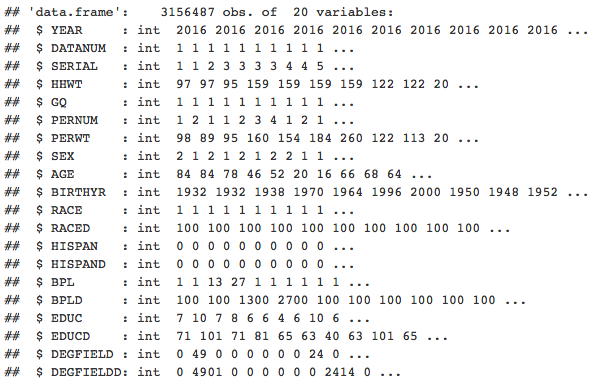
\includegraphics[width=1\textwidth]{data.png}
\caption{\label{fig:meritprograms}Internal structure of the data}
\end{figure}

\section{Methodology}
Following Sjoquist and Winters (2015), We employ a treatment and control, Difference-in-Difference strategy. Consistent with previous literature, exposure to treatment is determined by state of birth – if the respondent was born in a treatment state, they are assigned to treatment, if they were not born in a treatment state they are assigned to the control. Ideally, treatment should be assigned at time of graduation from high school, however the ACS data does not provide this information. As a result, there is some degree of measurement error. 

Using information from the Brookings Institution, Dynarski (2004), Heller (2004), and various state agency websites, Sjoquist and Winters (2015) categorize each state into one of three subsets: strong-merit states, weak-merit states, and no-merit states. The net assignment is nine strong-merit states, 18 weak-merit states, and 24 no-merit states (including Washington DC). The strong-merit states are believed to have a significant impact as measured by eligibility criteria, number of students and the magnitude of the award. Table 1 lists the characteristics (initial requirement, renewal requirements, etc.) of the nine strong-merit states. The weak-merit states were deemed insignificant and were not believed to have a meaningful impact on a student’s enrollment decision, let alone choice of major. 

\begin{figure}[!h]
\renewcommand{\floatpagefraction}{0.8}
\centering
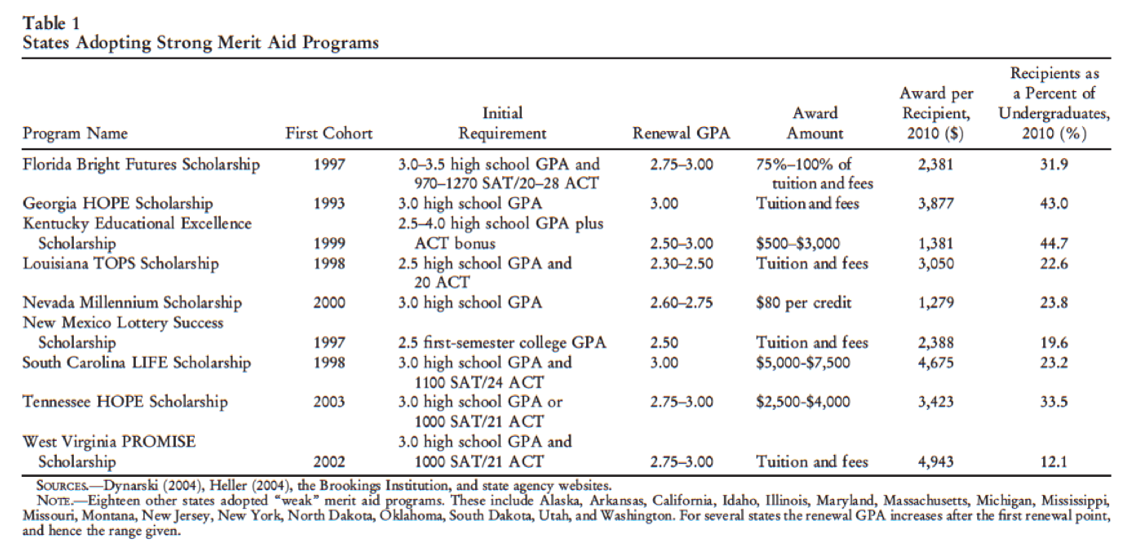
\includegraphics[width=1\textwidth]{meritprograms.png}
\caption{\label{fig:meritprograms}Strong-Merit Programs}
\end{figure}

The following linear probability model is employed:
P(Yisct = 1) = Γs + πc + βXisct + δsTsc + θMeritsc + εisct
Where Y equals one if individual i, from state s, born in cohort c, in survey year t, completed a bachelor’s degree in a STEM field; Γs is a state-of-birth fixed effect; πc is a birth cohort fixed effect; Xisct includes a set of dummy variables for age, Hispanic origin, race and sex; Tsc is a state-of-birth by year-of-birth time trend; and Meritsc is an indicator equal to one if the respondent was exposed to a state merit program. The parameter of interest is β and the inclusion of the state-of-birth and year-of-birth fixed effects allow β to be interpreted as a Difference-in-Differences estimate. It’s important to note that Meritsc is the interaction of a state and year variable. Given the ACS data is at the individual level, there will be intra-cluster correlation within each state. Standard errors are clustered at the state-of-birth level to account for this intra-cluster correlation. 

\begin{thebibliography}{9}
\bibitem{nano3}
  K. Grove-Rasmussen og Jesper Nygård,
  \emph{Kvantefænomener i Nanosystemer}.
  Niels Bohr Institute \& Nano-Science Center, Københavns Universitet

\end{thebibliography}

\begin{appendices}
\chapter
The results of the model are summarized here

\begin{center}
\begin{longtable}[!htbp]
\begin{tabular}
\\[-1.8ex]\hline 
\hline \\[-1.8ex] 
 & \multicolumn{1}{c}{\textit{Dependent variable:}} \\ 
\cline{2-2} 
\\[-1.8ex] & outstem \\ 
\hline \\[-1.8ex] 
 merit & $-$0.009 \\ 
  & (0.008) \\ 
  & \\ 
 race\_black & $-$0.050$^{***}$ \\ 
  & (0.006) \\ 
  & \\ 
 race\_asian & 0.160$^{***}$ \\ 
  & (0.007) \\ 
  & \\ 
 race\_other & $-$0.014 \\ 
  & (0.010) \\ 
  & \\ 
 hispanic & $-$0.022$^{***}$ \\ 
  & (0.006) \\ 
  & \\ 
 BIRTHYR\_1981 & 0.059 \\ 
  & (0.045) \\ 
  & \\ 
 BIRTHYR\_1980 & 0.057 \\ 
  & (0.045) \\ 
  & \\ 
 BIRTHYR\_1978 & 0.064 \\ 
  & (0.045) \\ 
  & \\ 
 BIRTHYR\_1988 & 0.055 \\ 
  & (0.045) \\ 
  & \\ 
 BIRTHYR\_1976 & 0.065 \\ 
  & (0.045) \\ 
  & \\ 
 BIRTHYR\_1977 & 0.072 \\ 
  & (0.045) \\ 
  & \\ 
 BIRTHYR\_1984 & 0.058 \\ 
  & (0.045) \\ 
  & \\ 
 BIRTHYR\_1971 & 0.044 \\ 
  & (0.045) \\ 
  & \\ 
 BIRTHYR\_1973 & 0.062 \\ 
  & (0.045) \\ 
  & \\ 
 BIRTHYR\_1990 & 0.087$^{*}$ \\ 
  & (0.045) \\ 
  & \\ 
 BIRTHYR\_1992 & 0.109$^{**}$ \\ 
  & (0.045) \\ 
  & \\ 
 BIRTHYR\_1970 & 0.053 \\ 
  & (0.045) \\ 
  & \\ 
 BIRTHYR\_1974 & 0.065 \\ 
  & (0.045) \\ 
  & \\ 
 BIRTHYR\_1972 & 0.046 \\ 
  & (0.045) \\ 
  & \\ 
 BIRTHYR\_1975 & 0.067 \\ 
  & (0.045) \\ 
  & \\ 
 BIRTHYR\_1986 & 0.058 \\ 
  & (0.045) \\ 
  & \\ 
 BIRTHYR\_1993 & 0.105$^{**}$ \\ 
  & (0.045) \\ 
  & \\ 
 BIRTHYR\_1982 & 0.063 \\ 
  & (0.045) \\ 
  & \\ 
 BIRTHYR\_1994 & 0.120$^{***}$ \\ 
  & (0.045) \\ 
  & \\ 
 BIRTHYR\_1979 & 0.059 \\ 
  & (0.045) \\ 
  & \\ 
 BIRTHYR\_1989 & 0.055 \\ 
  & (0.045) \\ 
  & \\ 
 BIRTHYR\_1987 & 0.067 \\ 
  & (0.045) \\ 
  & \\ 
 BIRTHYR\_1983 & 0.050 \\ 
  & (0.045) \\ 
  & \\ 
 BIRTHYR\_1991 & 0.093$^{**}$ \\ 
  & (0.045) \\ 
  & \\ 
 BIRTHYR\_1985 & 0.055 \\ 
  & (0.045) \\ 
  & \\ 
 BIRTHYR\_1995 & 0.130$^{***}$ \\ 
  & (0.049) \\ 
  & \\ 
 BIRTHYR\_1997 & 0.151$^{*}$ \\ 
  & (0.082) \\ 
  & \\ 
 BIRTHYR\_1996 &  \\ 
  &  \\ 
  & \\ 
 BPL\_1 & 0.060$^{***}$ \\ 
  & (0.023) \\ 
  & \\ 
 BPL\_12 & 0.037$^{*}$ \\ 
  & (0.022) \\ 
  & \\ 
 BPL\_13 & 0.033 \\ 
  & (0.023) \\ 
  & \\ 
 BPL\_22 & 0.059$^{**}$ \\ 
  & (0.023) \\ 
  & \\ 
 BPL\_36 & $-$0.005 \\ 
  & (0.020) \\ 
  & \\ 
 BPL\_48 & 0.031 \\ 
  & (0.020) \\ 
  & \\ 
 BPL\_28 & 0.036 \\ 
  & (0.025) \\ 
  & \\ 
 BPL\_17 & 0.029 \\ 
  & (0.020) \\ 
  & \\ 
 BPL\_47 & 0.024 \\ 
  & (0.023) \\ 
  & \\ 
 BPL\_8 & 0.067$^{***}$ \\ 
  & (0.022) \\ 
  & \\ 
 BPL\_19 & 0.018 \\ 
  & (0.023) \\ 
  & \\ 
 BPL\_37 & 0.024 \\ 
  & (0.022) \\ 
  & \\ 
 BPL\_34 & 0.005 \\ 
  & (0.021) \\ 
  & \\ 
 BPL\_6 & 0.021 \\ 
  & (0.020) \\ 
  & \\ 
 BPL\_27 & 0.044$^{**}$ \\ 
  & (0.022) \\ 
  & \\ 
 BPL\_18 & 0.058$^{***}$ \\ 
  & (0.022) \\ 
  & \\ 
 BPL\_21 & 0.014 \\ 
  & (0.023) \\ 
  & \\ 
 BPL\_29 & 0.027 \\ 
  & (0.022) \\ 
  & \\ 
 BPL\_41 & 0.026 \\ 
  & (0.024) \\ 
  & \\ 
 BPL\_15 & $-$0.003 \\ 
  & (0.027) \\ 
  & \\ 
 BPL\_39 & 0.039$^{*}$ \\ 
  & (0.021) \\ 
  & \\ 
 BPL\_45 & 0.015 \\ 
  & (0.024) \\ 
  & \\ 
 BPL\_9 & 0.002 \\ 
  & (0.022) \\ 
  & \\ 
 BPL\_32 & 0.110$^{***}$ \\ 
  & (0.032) \\ 
  & \\ 
 BPL\_49 & 0.056$^{**}$ \\ 
  & (0.023) \\ 
  & \\ 
 BPL\_35 & 0.086$^{***}$ \\ 
  & (0.027) \\ 
  & \\ 
 BPL\_5 & 0.050$^{**}$ \\ 
  & (0.025) \\ 
  & \\ 
 BPL\_55 & 0.074$^{***}$ \\ 
  & (0.022) \\ 
  & \\ 
 BPL\_42 & 0.037$^{*}$ \\ 
  & (0.020) \\ 
  & \\ 
 BPL\_23 & 0.117$^{***}$ \\ 
  & (0.028) \\ 
  & \\ 
 BPL\_31 & 0.036 \\ 
  & (0.025) \\ 
  & \\ 
 BPL\_40 & 0.044$^{*}$ \\ 
  & (0.023) \\ 
  & \\ 
 BPL\_26 & 0.065$^{***}$ \\ 
  & (0.021) \\ 
  & \\ 
 BPL\_11 & 0.039 \\ 
  & (0.026) \\ 
  & \\ 
 BPL\_33 & 0.056$^{**}$ \\ 
  & (0.028) \\ 
  & \\ 
 BPL\_54 & 0.063$^{**}$ \\ 
  & (0.026) \\ 
  & \\ 
 BPL\_25 & 0.014 \\ 
  & (0.021) \\ 
  & \\ 
 BPL\_51 & 0.052$^{**}$ \\ 
  & (0.022) \\ 
  & \\ 
 BPL\_20 & 0.051$^{**}$ \\ 
  & (0.024) \\ 
  & \\ 
 BPL\_24 & 0.054$^{**}$ \\ 
  & (0.022) \\ 
  & \\ 
 BPL\_53 & 0.041$^{*}$ \\ 
  & (0.022) \\ 
  & \\ 
 BPL\_2 & 0.072$^{**}$ \\ 
  & (0.035) \\ 
  & \\ 
 BPL\_38 & 0.120$^{***}$ \\ 
  & (0.030) \\ 
  & \\ 
 BPL\_4 & 0.037 \\ 
  & (0.023) \\ 
  & \\ 
 BPL\_16 & 0.062$^{**}$ \\ 
  & (0.028) \\ 
  & \\ 
 BPL\_46 & 0.096$^{***}$ \\ 
  & (0.030) \\ 
  & \\ 
 BPL\_10 & 0.044 \\ 
  & (0.031) \\ 
  & \\ 
 BPL\_56 & 0.101$^{***}$ \\ 
  & (0.036) \\ 
  & \\ 
 BPL\_30 & 0.143$^{***}$ \\ 
  & (0.030) \\ 
  & \\ 
 BPL\_50 & 0.050 \\ 
  & (0.033) \\ 
  & \\ 
 BPL\_44 &  \\ 
  &  \\ 
  & \\ 
 Constant & 0.206$^{***}$ \\ 
  & (0.048) \\ 
  & \\ 
\hline \\[-1.8ex] 
Observations & 119,892 \\ 
R$^{2}$ & 0.009 \\ 
Adjusted R$^{2}$ & 0.009 \\ 
Residual Std. Error & 0.459 (df = 119809) \\ 
F Statistic & 14.009$^{***}$ (df = 82; 119809) \\ 
\hline 
\hline \\[-1.8ex] 
\textit{Note:}  & \multicolumn{1}{r}{$^{*}$p$<$0.1; $^{**}$p$<$0.05; $^{***}$p$<$0.01} \\ \end{tabular} \end{longtable} 
\end{appendices}
\end{document}